\documentclass[notes,compress,sanserif,professionalfont]{beamer}
\usetheme{boxes} %Boadilla, Berkeley, Dresden, Rochester, Pittsburgh
\useoutertheme{miniframes} %split, shadow, infolines, default
\usepackage{hyperref}
\usepackage{pxfonts}
\usepackage{amsmath}
\usepackage{amssymb}
\usepackage{amsfonts}
\usepackage{enumerate}
\usepackage{natbib}
\usepackage{xcolor}
\usepackage{multirow}
\usepackage{tikz}
\usepackage{subfigure}
\usetikzlibrary{arrows,shapes}
\usepackage{bbding} % for \Checkmark symbol
\beamertemplateballitem % make bullets and items fancy balls
\useheadtemplate{%
\vbox{%
\vskip1pt%
\beamerline{\insertnavigation{\paperwidth}}%
%\vskip-5pt   %to place frametitles closer to the navigation bar
}
}
%\renewcommand{\frametitle}[1]{\begin{center}\textbf{#1}\end{center}}
% Define local notation.

\def\etal{{\emph{et alia\/}}}
\def\sR{\textsf{R}}
\def\argmax{\mathop{\rm argmax}}
\def\cL{{\cal L}}


% \AtBeginSection[]
% {
%     \begin{frame}
%         \frametitle{Outline}
%         \tableofcontents[currentsection]
%     \end{frame}
% }
\AtBeginSection[]{
  \begin{frame}
  \vfill
  \centering
  \begin{beamercolorbox}[sep=8pt,center,shadow=true,rounded=true]{title}
    \usebeamerfont{title}\insertsectionhead\par%
  \end{beamercolorbox}
  \vfill
  \end{frame}
}

\begin{document}
\title{Selecting the Optimal Credit Card Portfolio}
\subtitle{Part 2: Data Sources}
\author{Remco A.~Scheepmaker}
\date{17 June 2024}

\begin{frame}
  \titlepage
\end{frame}

% Presentation 2 (June 17): Presentation of the outline paper, including data sources and how I plan to solve the problem using the data.

% \begin{frame}
%     \frametitle{ }
%     \begin{quote}
%         \centerline{In 30 minutes\ldots}
%         \vskip 16pt
%         \centerline{you'll know how to be financially sophisticated}
%         \centerline{and profit from the financially na\"{i}ve!}
%     \end{quote}
% \end{frame}

\begin{frame}{Outline}
    \tableofcontents
\end{frame}

\section{Recap}

\subsection{Research Questions}

\begin{frame}{Research Questions}
    \begin{itemize}
        \item Credit cards reward the user with spend (cash back or points), and might have static benefits (lounge access, travel/food credit, etc.), and annual fees
        \bigskip
        \item To maximize the net benefit, how should a financially sophisticated cardholder optimize her credit card portfolio?
        \bigskip
        \item What is the value?
        \bigskip
        \item How does this value change with number of cards, income, and user preferences?
    \end{itemize}
\end{frame}    

\subsection{Empirical Specification}

\begin{frame}{Empirical Specification}
Total net benefit of the portfolio:
    \[
        Y(\mathbf{X}, K, \eta, \theta | \mathbf{M}, \mathbf{v_{t}}, \mathbf{v_{b}}, \mathbf{b}, \mathbf{f} ) = \sum_{k=1}^{K}\left( s_{k} + \theta\/ b_{k} - f_{k}\right),
    \]
where (value of spend on card $k$)
\[
    s_{k} = \sum_{c=1}^{C}y_{kc},
\]
and (value of spend of card $k$ on category $c$)
\[
    y_{kc} = x_{kc}\/m_{kc} \left[ \eta\/ v_{t,k} + 
    (1 - \eta)\/ v_{b,k}\right].
\]
\end{frame}    

\begin{frame}{Data Needed}
    \begin{itemize}
        \item Card Parameters
        \begin{itemize}
            \item Point multipliers and limits ($k\times c$ matrix $\mathbf{M}$)
            \item Base and travel values of the points (vectors $\mathbf{v_{b}}$ and $\mathbf{v_{t}}$)
            \item Benefits and fees (vectors $\mathbf{b}$ and $\mathbf{f}$)
        \end{itemize}
        \bigskip
        \item User Variables
        \begin{itemize}
            \item Budget matrix $\mathbf{X}$ (depends on income!)
            \item Number of cards $K$
            \item Preferences (travel redemptions $\eta$ and benefits $\theta$)
        \end{itemize}
    \end{itemize}
\end{frame}

\section{Credit Card Data}

\subsection{Spending Categories}

\begin{frame}{Spending Categories}
    \begin{columns}[c]
        \begin{column}{0.4\textwidth}
            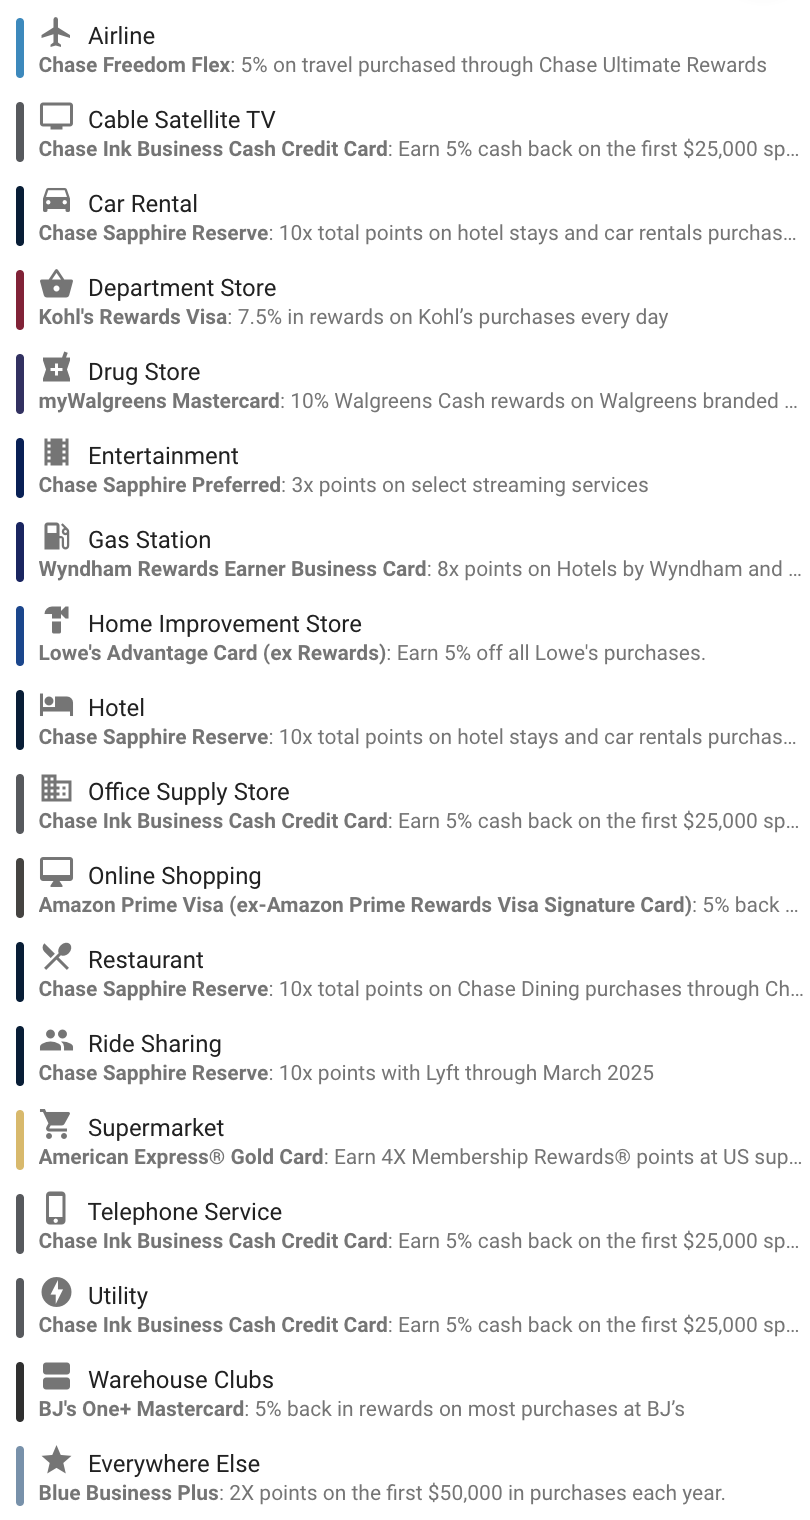
\includegraphics[scale=0.3]{../Misc/CardPointersCategories.png}
        \end{column}
        \begin{column}{0.6\textwidth}
            \begin{itemize}
                \item 18 categories from \url{https://cardpointers.com/app/}
                \item Removed ``Warehouse Clubs'' and ``Ride Sharing'' 
                \item Added ``Streaming'' and ``Travel (other)''
            \end{itemize}
        \end{column}
    \end{columns}
\end{frame}

\subsection{Multipliers \& Point Values}

\begin{frame}{Credit Card Selection}
    \begin{itemize}
        \item Selected 28 rewards credit cards from 7 major banks
        \begin{itemize}
            \item American Express, Chase, Bank of America, Citi, Capital One, US Bank, and Wells Fargo
        \end{itemize}
        \smallskip

        \item Since we work with an \emph{average} spending budget
        \begin{itemize}
            \item Ignore cards from stores, hotels, airlines
            \item Ignore cards with \emph{exotic} categories (``mobile wallets'')
            \item Ignore cards with \emph{variable} (quarterly) categories
        \end{itemize}
        \smallskip
        \item But create duplicates of cards with \emph{custom} categories
        \begin{itemize}
            \item Prototype model contains 38 cards
        \end{itemize}
   \end{itemize}
\end{frame}

\begin{frame}{Point Multipliers}
    Example from \url{https://www.allcards.com/travel-reward-credit-cards/}
    \begin{center}
        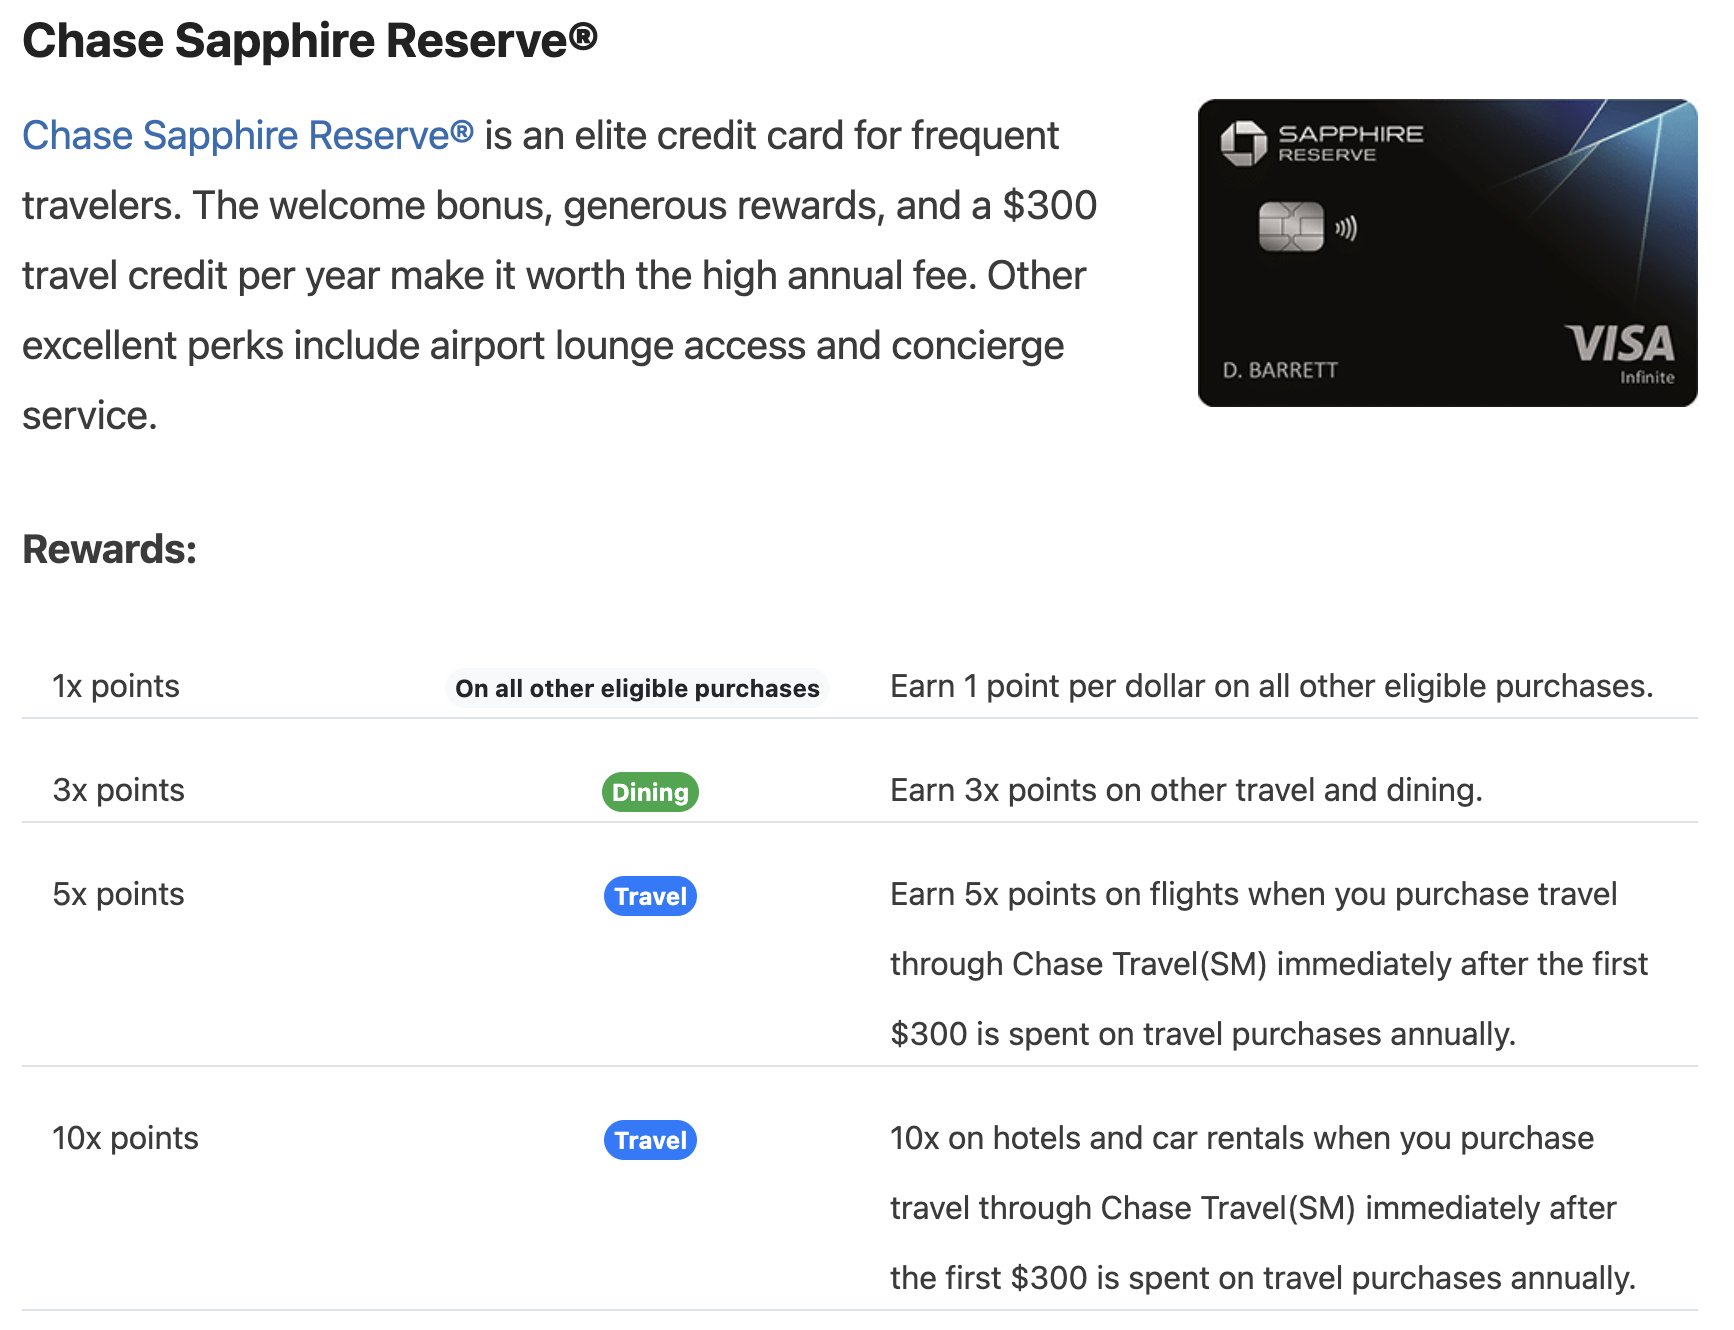
\includegraphics[width=.8\textwidth]{../Misc/AllcardsExample.png}
    \end{center}
\end{frame}

\begin{frame}{Point Values}
    \begin{itemize}
        \item Taken from \citet{nerdwallet:2024}\footnote{\url{https://www.nerdwallet.com/article/travel/airline-miles-and-hotel-points-valuations}}
        \begin{center}
            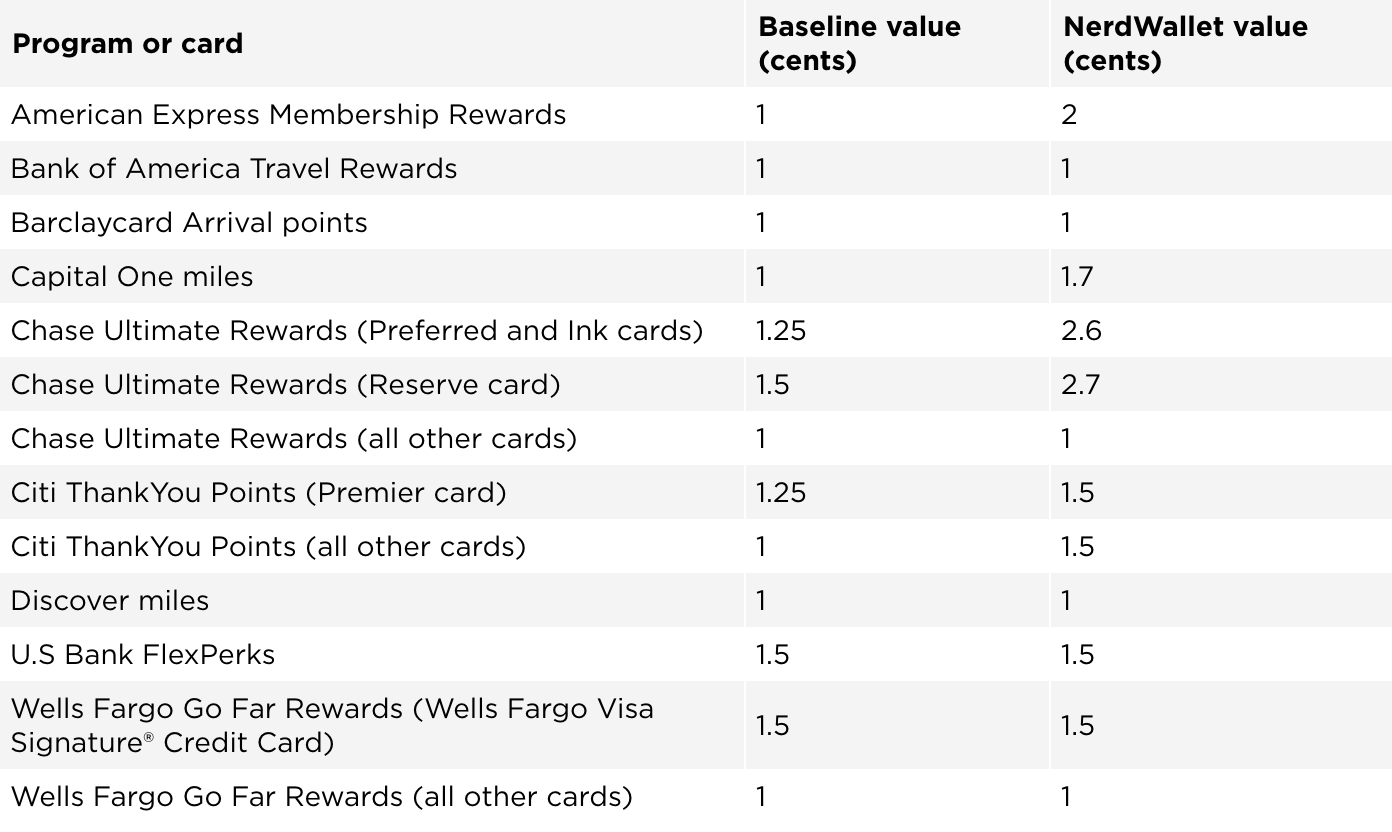
\includegraphics[width=.8\textwidth]{../Misc/PointValuesNerdwallet.png}
        \end{center}
        \item I will ignore advanced strategies for now (Bi- and Trifectas, Bank of America Preferred Rewards)
    \end{itemize}
\end{frame}


\subsection{Benefits}

\begin{frame}{Static Benefits}
\begin{columns}[c]
    \begin{column}{0.6\textwidth}
        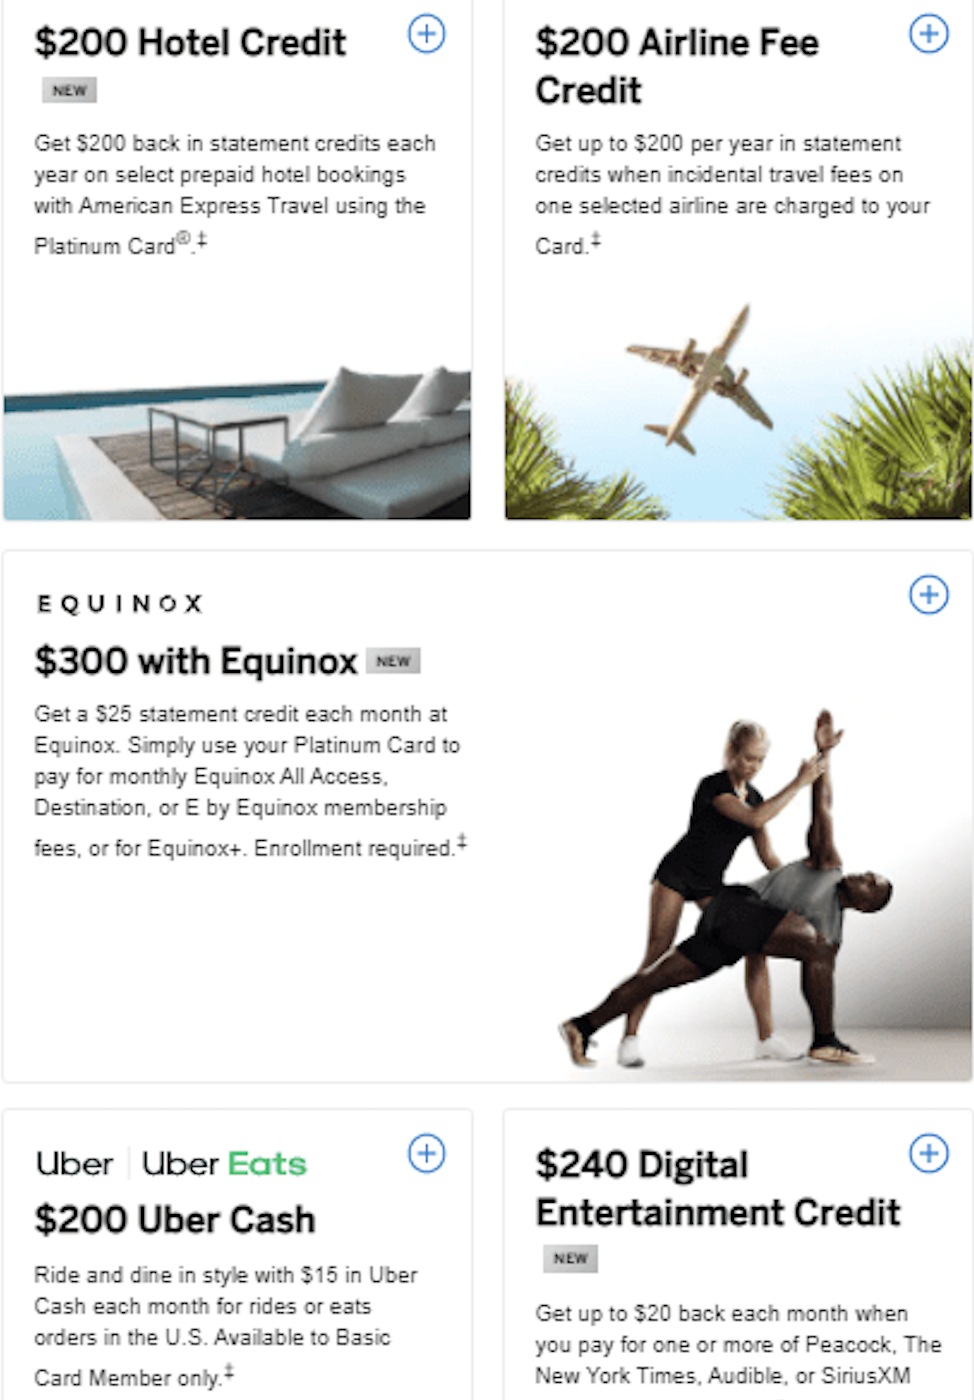
\includegraphics[height=0.9\textheight]{../Misc/AmexPlatinum.png}
    \end{column}
    \begin{column}{0.4\textwidth}
        \centering
        These are the most difficult to quantify! 
        (extreme example:\\ Amex Platinum)
    \end{column}
\end{columns}
\end{frame}

\begin{frame}{Static Benefits}
    \begin{itemize}
        \item Are also controlled by the $\theta$ parameter
        \item Will have to use my judgment on what ``reasonable'' benefits are:
        \begin{itemize}
            \item Lounge access: \$40 per year
            \item Global Entry / TSA Pre\Checkmark: \$20 per year
            \item Clear: \$189 per year
            \item Travel and food credits: full value 
        \end{itemize}
        \item Ideally, in an online tool these can be adjusted by the user
    \end{itemize}
\end{frame}

\begin{frame}{Final (partial) Dataset}
    \begin{center}
        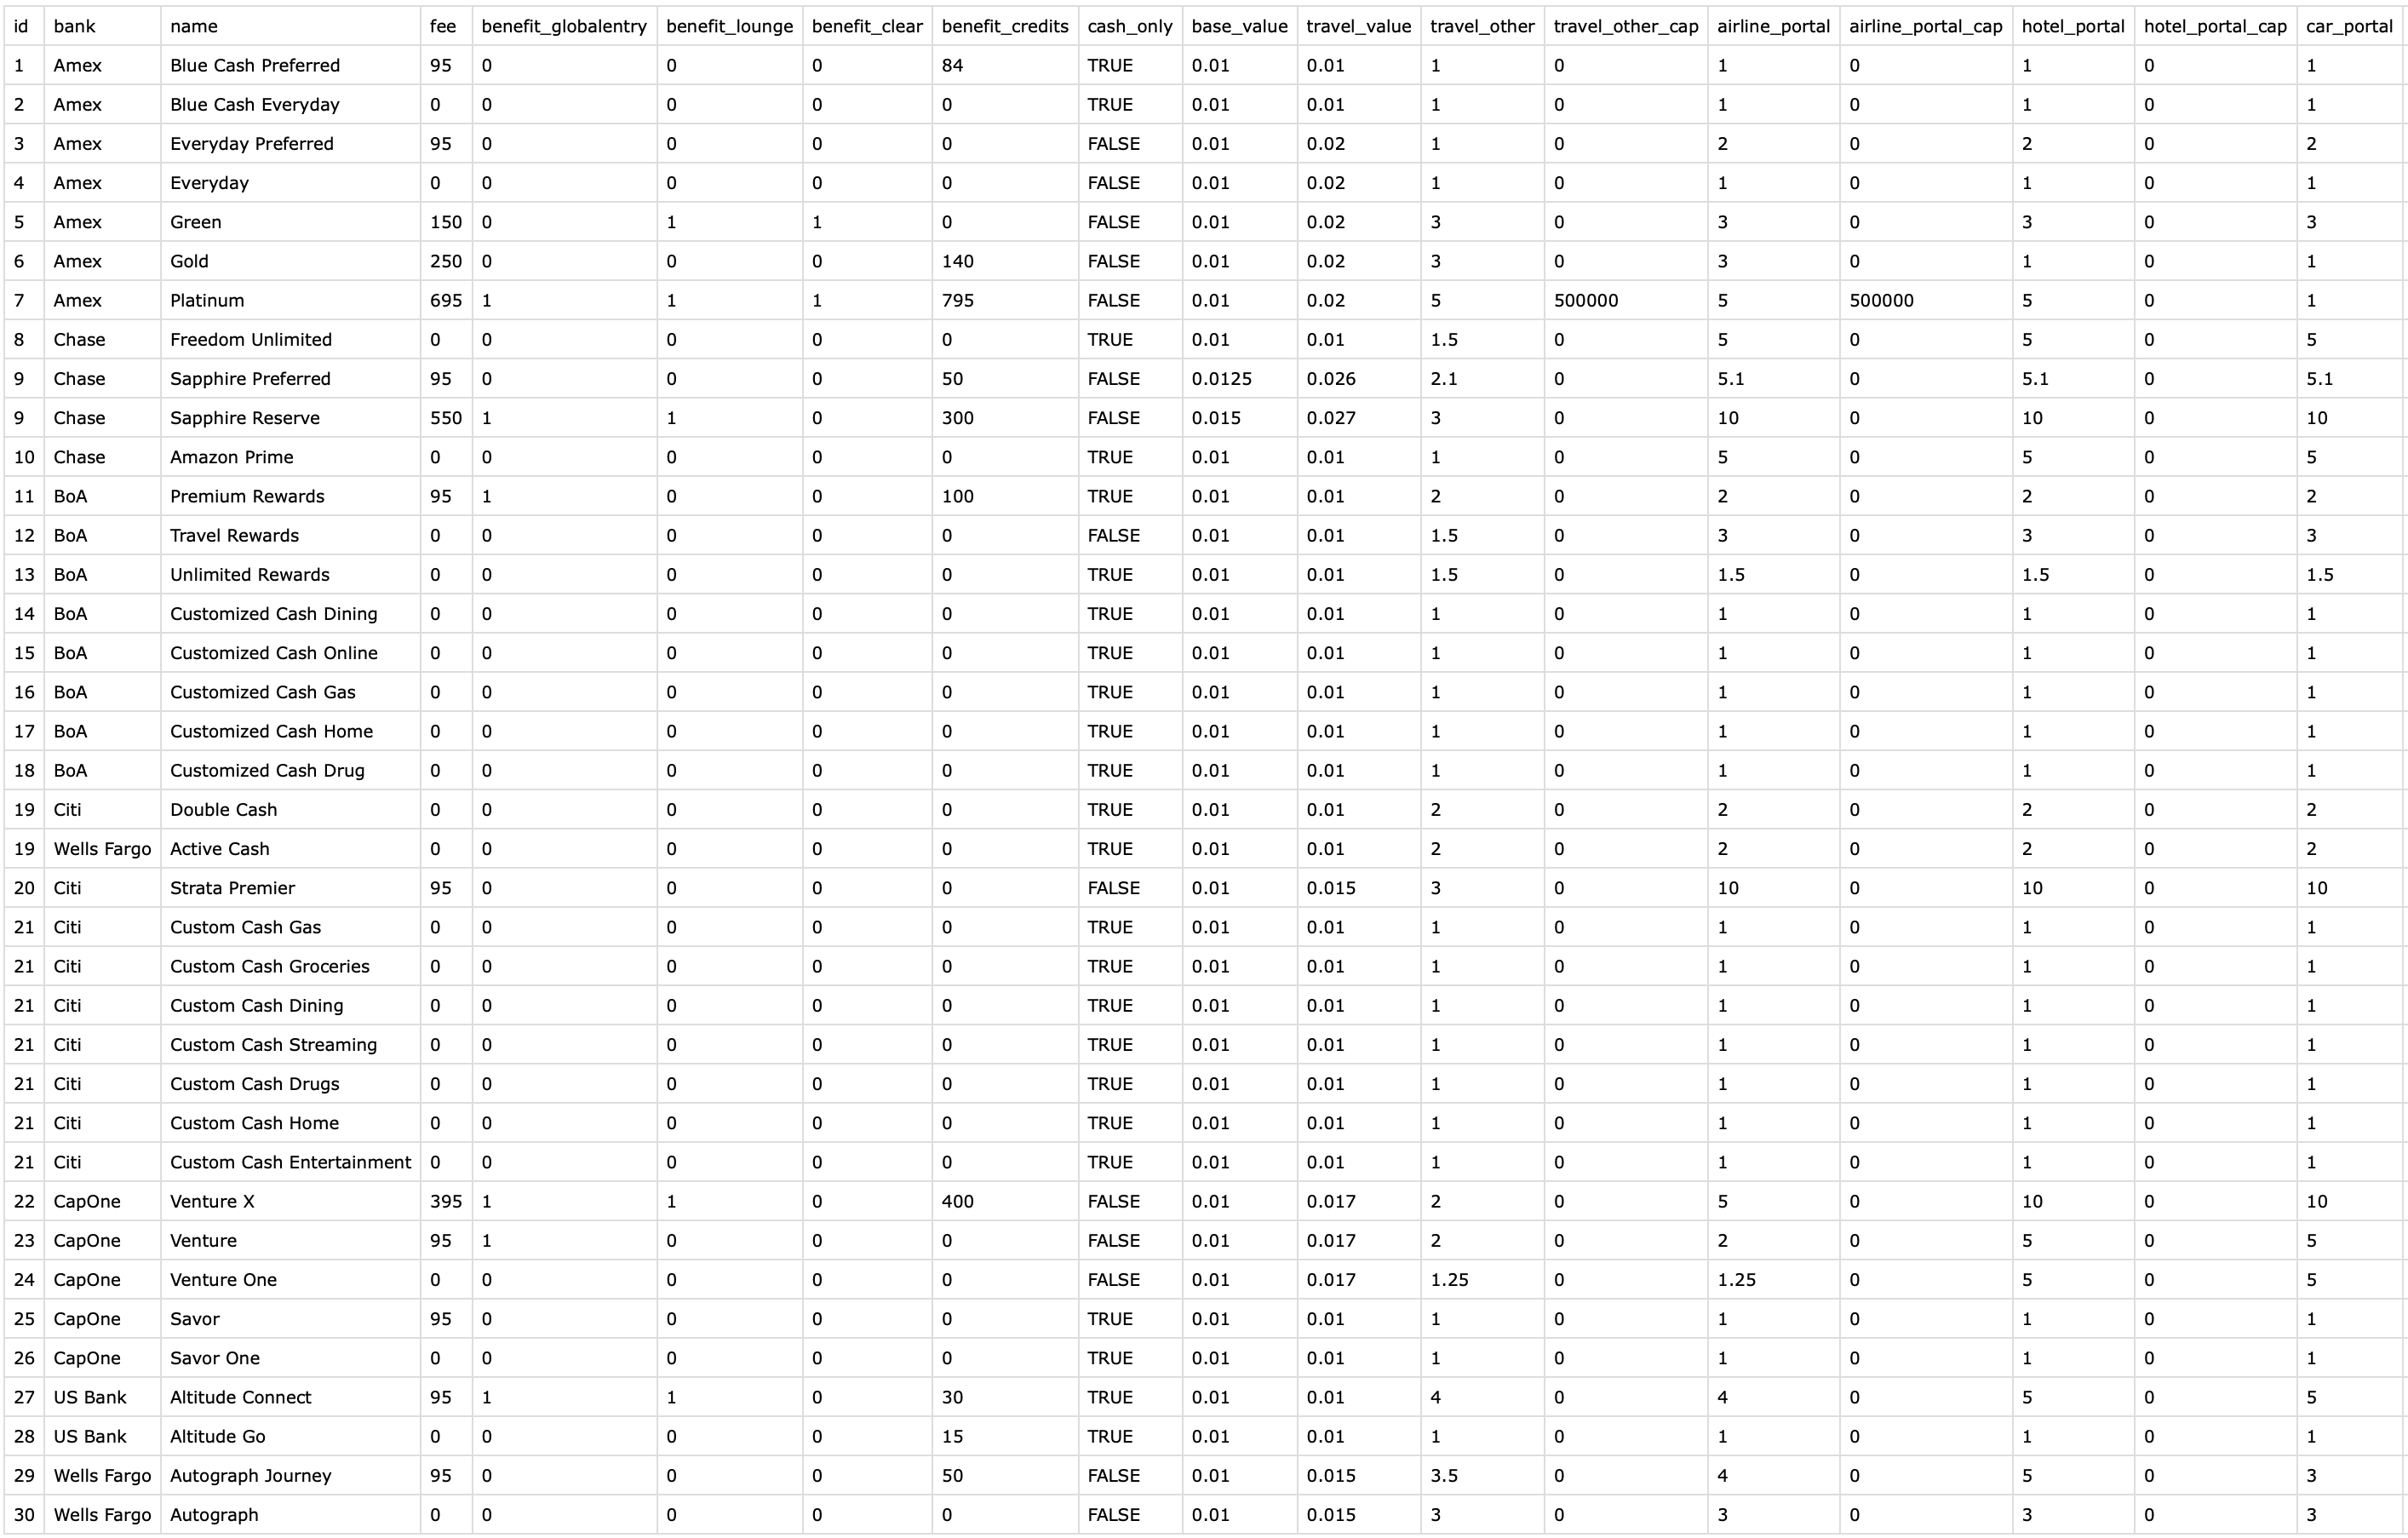
\includegraphics[width=1.0\textwidth]{../Misc/CreditCardsCSV.png}
    \end{center}
\end{frame}

\section{User Data}

\subsection{Mean Spending Budget}

\begin{frame}{Consumer Expenditure Survey (CES)}
    \begin{itemize}
        \item Mean expenditures from the 2022 CES: \$72,967 from income of \$94,003 \citep{bls:2023}
        \bigskip
        \item Subtracted shelter, vehicle purchases, health insurance, education, cash contributions, personal insurance, and pensions
        \bigskip
        \item Remaining \$38,576 of expenditures (41\% of income) were mapped to the 18 credit card categories
    \end{itemize}
\end{frame}

\begin{frame}{Average Spending Budget}
    \begin{itemize}
        \item Note: some items were split over two categories
    \end{itemize}
    \begin{center}
        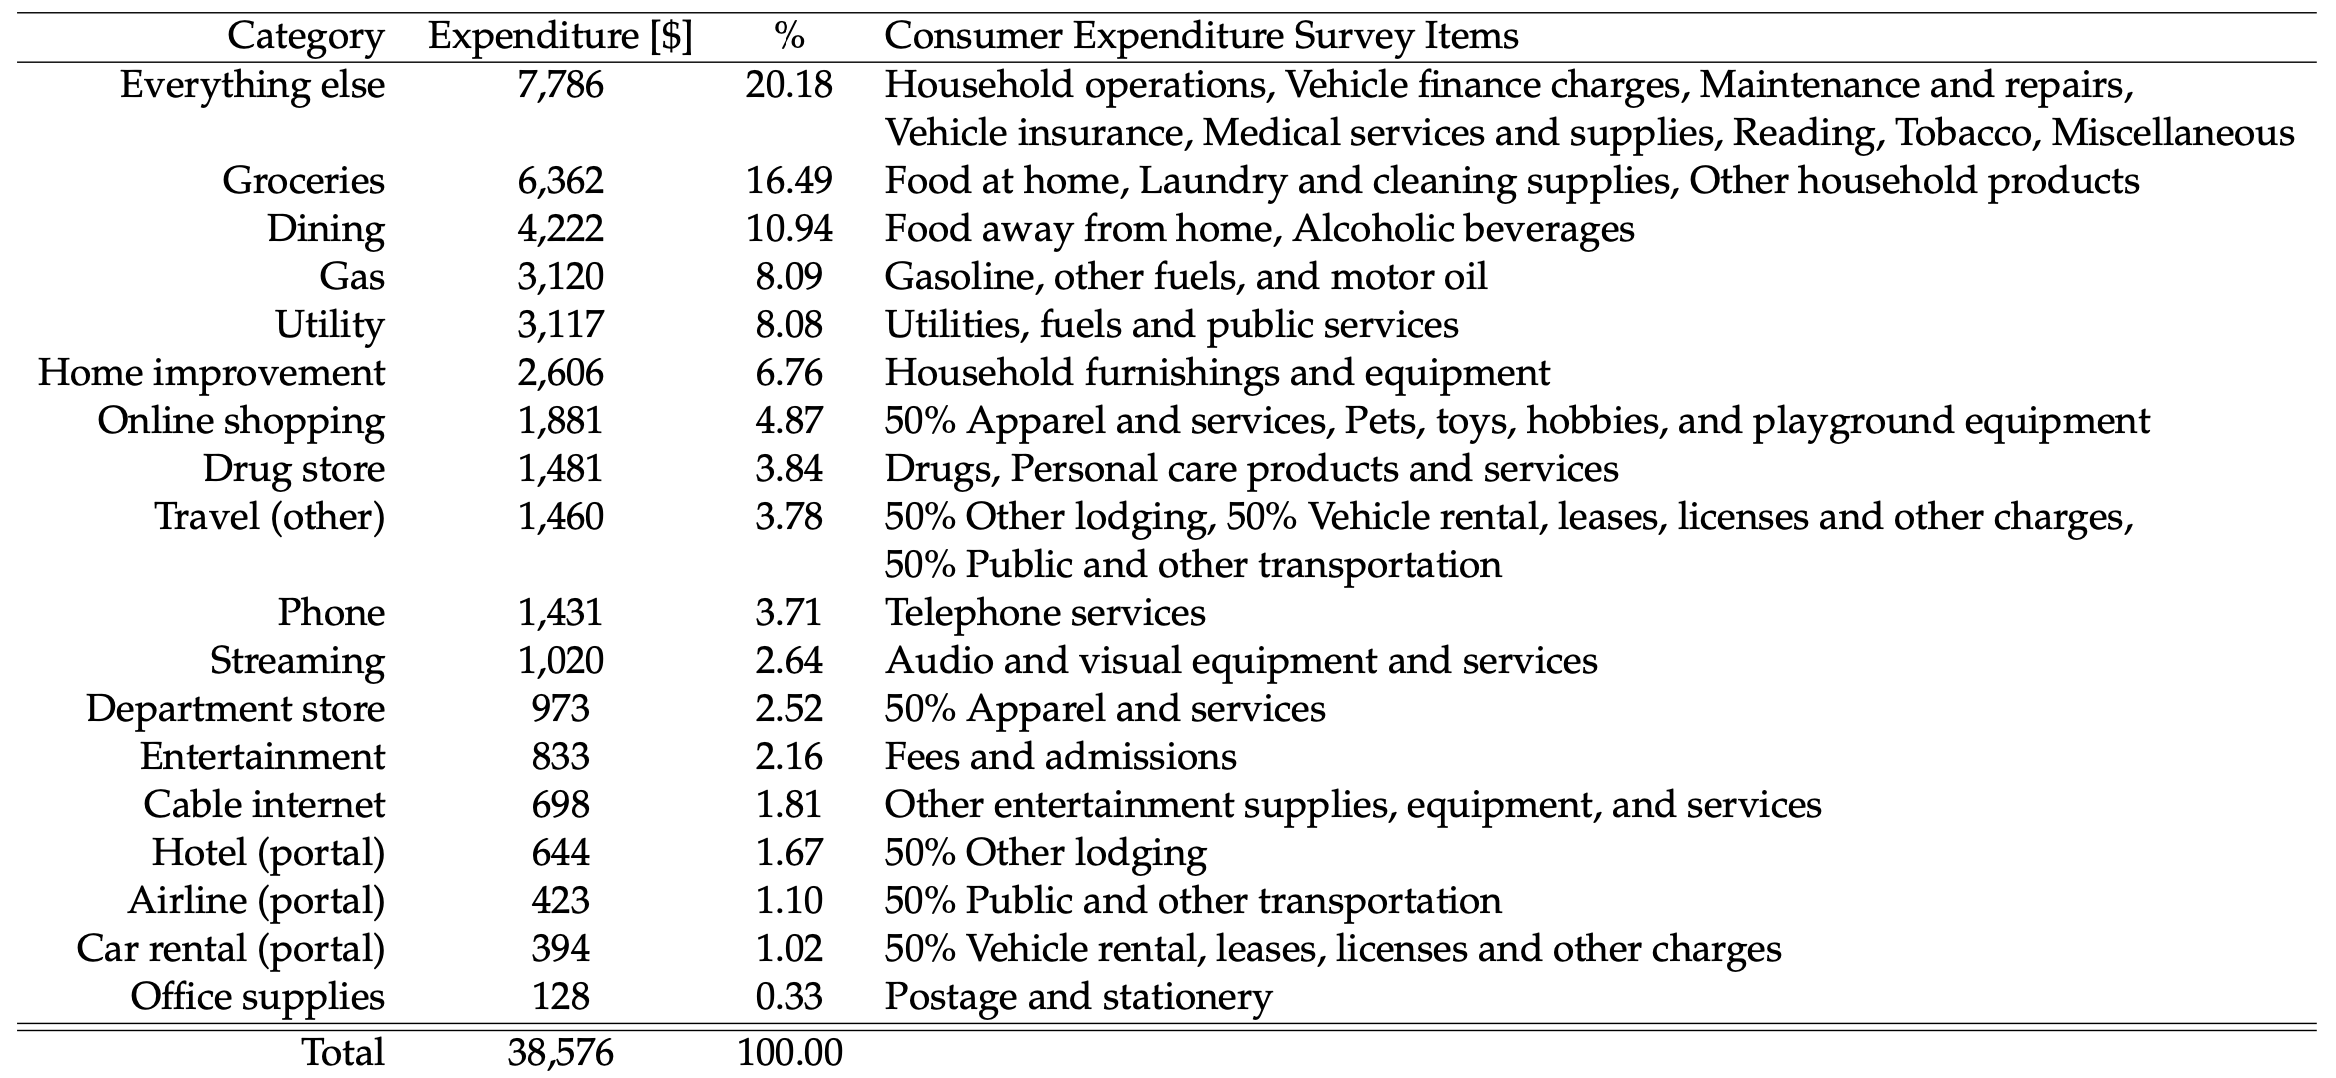
\includegraphics[width=\textwidth]{../Misc/BudgetExtended.png}
    \end{center}
\end{frame}

\subsection{Income \& Preferences}

\begin{frame}{Income \& Preferences}
    \begin{itemize}
        \item Make the budget dependent on 9 income bins (done!)
        \begin{itemize}
            \item Initially assume \$94k (CES mean), \$45k, and \$160k
        \end{itemize}
        \bigskip
        \item ``Transfer redemptions'' $\eta$ and ``use of benefits'' $\theta$
        \begin{itemize}
            \item Initially assume $\eta, \theta \; \in \; [0, 0.5, 1.0]$
        \end{itemize}
        \bigskip
        \item If successful, attempt Monte-Carlo Simulations
        \begin{itemize}
        \item Sample income from observed distribution (U.S. Census)
        \item Sample $\eta, \theta$ from uniform distributions
        \end{itemize}
        \bigskip
        \item Ultimate goal: an online tool with user input (including personal budget!)
   \end{itemize}
\end{frame}

\begin{frame}{Income Dependent Budgets}
    \begin{center}
        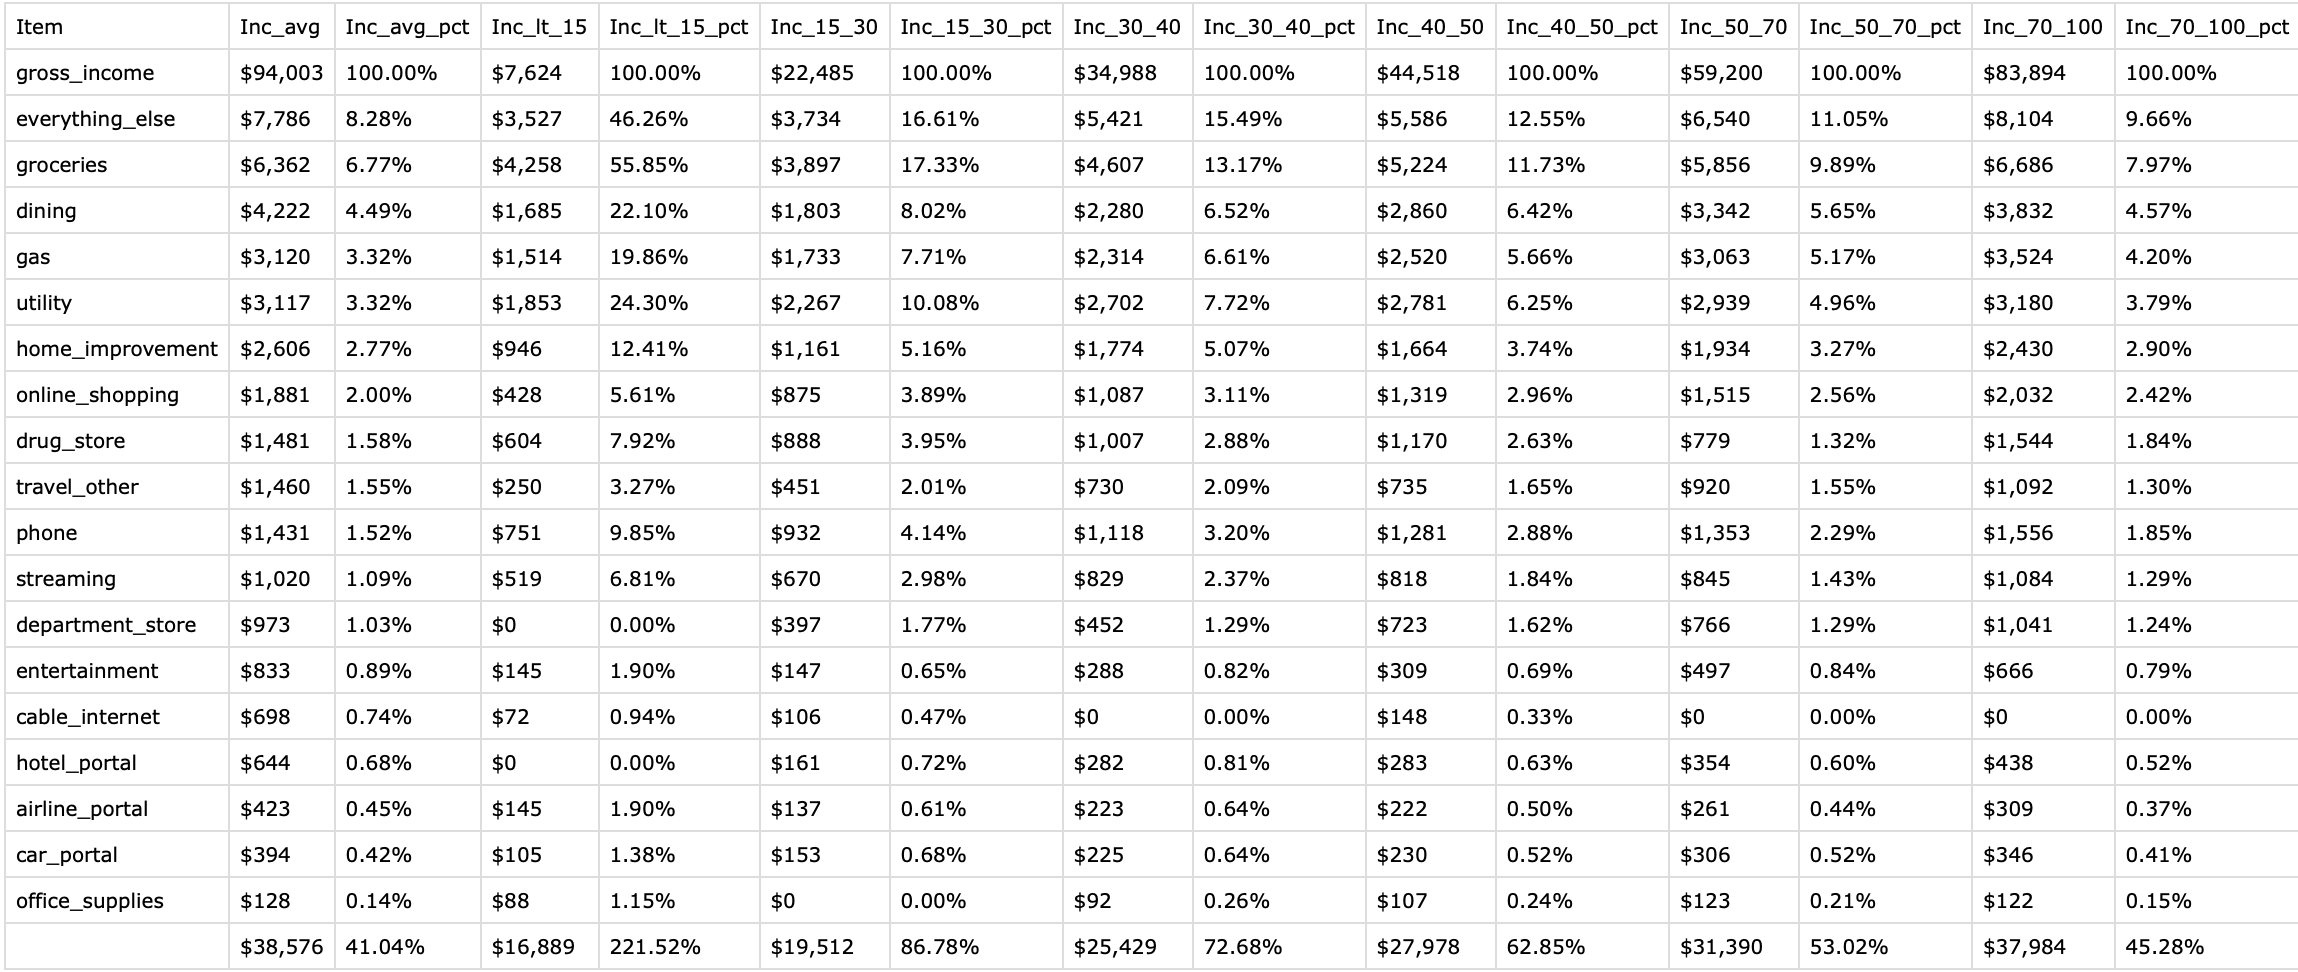
\includegraphics[scale=0.4]{../Misc/BudgetIncome.png}
    \end{center}
\end{frame}


\section{Next Steps}

\begin{frame}{Next Steps}
    \begin{itemize}
        \item Finish income-dependent budgets (actually, it's done!)
        \bigskip
        \item Start coding the optimization algorithm in R
        \bigskip
        \item Plan the visualizations and tables I need
        \bigskip
        \item Look into sampling incomes from the observed distribution
    \end{itemize}
\end{frame}   

\begin{frame}
    \vfill
    \centering
    \begin{beamercolorbox}[sep=8pt,center,shadow=true,rounded=true]{title}
      \usebeamerfont{title}Thank You!
    \end{beamercolorbox}
    \vfill
\end{frame}


% WILL HAVE TO CHANGE BUDGET TO AVERAGE +9 INCOME BINS,
% AND MAKE THEM PERCENTAGES OF INCOME BEFORE TAXES!

% \section{Summary \& Conclusions}

% \begin{frame}{Summary \& Conclusions}
%     \begin{itemize}
%         \item Bla 1
%         \bigskip
%         \item Bla 2
%         \bigskip
%         \item Bla 3!
%     \end{itemize}
% \end{frame}   

\begin{frame}{References}
    \bibliographystyle{../chicago}
    \bibliography{../References}
\end{frame}    


%\begin{appendix}
\section{Data Appendix}
\begin{frame}
\frametitle{Data Appendix}
\begin{itemize}

\item 1.
\item 2.
\item 3.

\end{itemize}
\end{frame}
\end{appendix}


\end{document}
